\documentclass[10pt]{article}
\usepackage[margin=0.75in]{geometry}
\usepackage{amsmath,booktabs,tabularx,pgfplots}
\usepackage[hidelinks]{hyperref}
\pgfplotsset{compat=1.18}
\setlength{\parindent}{0pt}
\setlength{\parskip}{5pt}
\title{Conformal Winner Sets: A First Evaluation}
\author{}\date{2026-11-06}
\begin{document}
\maketitle
\vspace{-2em}

\section{Setup}

I took the finished model, and the unused test matches, splitting it 67 calibration matches, 67 evaluation matches. I took a single nonterminal prefix per match to evaluate.

\section{Method}

I used split conformal prediction with score $s_i=1-p(y_i\mid x_i)$ and the $k=\lceil(n+1)(1-\alpha)\rceil$th ordered calibration score $q$. If $k>n$, both teams are included.
I used $\alpha = 0.1$. See \href{https://arxiv.org/abs/2107.07511}{Angelopoulos and Bates} for the method I used. 

\begin{center}\small
\begin{tabularx}{0.95\linewidth}{Xr}
\toprule
Statistic & Evaluation result \\
\midrule
Nominal / observed coverage & 90\% / 92.5\% \\
Observed coverage, descriptive 95\% Wilson interval & [83.7\%, 96.8\%] \\
Quantile rank / calibration count; threshold $q$ & 62 / 67; 0.665159 \\
Mean prediction-set size (maximum 2) & 1.672 \\
Empty / singleton / two-team sets & 0 / 22 / 45 \\
Accuracy among singleton sets & 77.3\% \\
Original model's argmax accuracy & 59.7\% \\
\bottomrule
\end{tabularx}\end{center}

\begin{center}
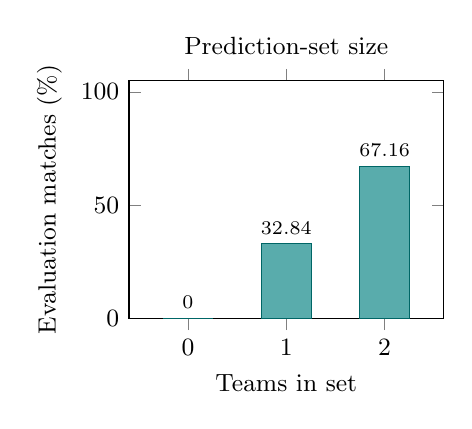
\begin{tikzpicture}
\begin{axis}[width=0.46\textwidth,height=4.6cm,ybar,bar width=18pt,
title={Prediction-set size},xlabel={Teams in set},ylabel={Evaluation matches (\%)},
xtick={0,1,2},ymin=0,ymax=105,enlarge x limits=0.3,
tick label style={font=\small},label style={font=\small},title style={font=\small},
nodes near coords,nodes near coords style={font=\scriptsize}]
\addplot[fill=teal!65,draw=teal!80!black] coordinates {(0,0.000000) (1,32.835821) (2,67.164179)};
\end{axis}
\end{tikzpicture}\hfill
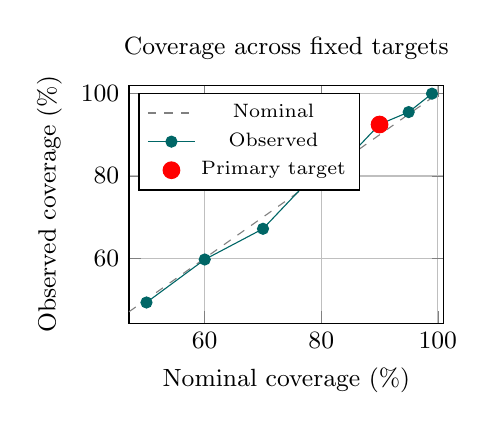
\begin{tikzpicture}
\begin{axis}[width=0.46\textwidth,height=4.6cm,
title={Coverage across fixed targets},xlabel={Nominal coverage (\%)},ylabel={Observed coverage (\%)},
xmin=47.00,xmax=101,ymin=44.25,ymax=102,grid=major,
tick label style={font=\small},label style={font=\small},title style={font=\small},
legend style={font=\scriptsize,at={(0.03,0.97)},anchor=north west}]
\addplot[gray,dashed] coordinates {(47.00,47.00) (100,100)};
\addlegendentry{Nominal}
\addplot[teal!80!black,mark=*] coordinates {(50.000000,49.253731) (60.000000,59.701493) (70.000000,67.164179) (80.000000,82.089552) (85.000000,85.074627) (90.000000,92.537313) (95.000000,95.522388) (99.000000,100.000000)};
\addlegendentry{Observed}
\addplot[red,only marks,mark=*,mark size=3pt] coordinates {(90,92.5)};
\addlegendentry{Primary target}
\end{axis}
\end{tikzpicture}
\end{center}
{\small AI-Generated summary table.}

\section{Results}

At the 90\% target, the sets contained the winner in 62 of 67 evaluation matches (92.5\%). it had one team in 22 matches and both in 45. Accuracy among singletons 
is an informative statistic, it tells us about the confidence of the model.

\section{Conclusion}

I would like to try using more matches, and see how it improves. Also, some of these matches may have shared players or been across different patches, so that may hurt the 
gaurantees of exchangability. I also want to check how these set size plots change over time, as it should be a monotonic decrease in set size over time.

\end{document}